\documentclass[../3Wworkreport.tex]{subfiles}
\doublespacing

\begin{document}

\section{Analysis}
\label{sec:analysis}

To capitalize on the ideas provided by quantum mechanics, one can associate the $d$-dimensional vector $x$ with the $d$-dimensional qudit $\ket{\psi}$, and let $x$ be the mathematical representation of $\ket{\psi}$. In doing this, some mathematical tools used in discrete quantum systems, such as the discrete Wigner function (\Cref{app:dwf}), become useful in solving Raz\rq{}s problems. By adapting the protocol outlined by Pashayan et al. \parencite*{Pashayan2014} for each problem, one can arrive at some classical computational protocols that solve Raz\rq{}s problems probabilistically. These adapted protocols are more technical in nature, and are given in \Cref{app:protocol1,app:protocol2}. It is highly recommended that the reader review these appendices in order to follow the complexity analysis in the following subsections.\\

A key point to note is that throughout both of these protocols, no quantum computation ever occurs. These solutions are inspired by the stabilizer sub-theory, which behaves differently than general quantum computation. Additionally, calculating $\hat{x}$ between Step 5 and Step 6 in Protocol 1 (and similarly calculating $\hat{v}$ between Step 6 and Step 7 in Protocol 2) can be done since the vectors $x$ and $Ux$ are real (and thus $\ket{\psi}$ and $U\ket{\psi}$ are as well). If one was to perform a basis measurement on $\ket{\psi}$ and $O$ is the random variable associated with the measurement outcome, then $O$ is associated with the distribution Pr$(O = k) = |\braket{\psi|k}|^2$. The value of the probability is the square of the $k$th component of $\ket{\psi}$. Computing the sample probability Pr($O = k$) approximates the value of the $k$th element of $x$ in Protocol 1. Doing this for each $k$ produces the values of the vector $\hat{x}$. The same idea holds for $U\ket{\psi}$ and the $k$th value of $Ux$ in Protocol 2, using Pr$(O = k) = |\Braket{\psi |U|k}|^2$.

\vspace{-0.5cm}
\subsection{Convergence and Repetition of the Protocols}
\label{subsec:convergence_repetitions}
The sample average, $\hat{R}$, over $T$ repetitions, obeys the Chernoff-Hoeffding inequality \parencite{Pashayan2014}:
\begin{equation}
	\text{Pr}(|\hat{R} - \mathbb{E}(R)|) \ge \epsilon) \le 2e^{\frac{-T\epsilon^2}{2\mathcal{M}^2}} \label{eq:chernoff}
\end{equation}
where $\mathcal{M} = \mathcal{M}_\rho\mathcal{M}_U$, the total mana of the system (\Cref{app:dwf}). Thus, if $T$ is large enough for each solution, then probabilistic convergence is guaranteed. In order to determine $T$, finding an upper bound for $\mathcal{M}$ is required. This value of $\mathcal{M}$ depends on $x$ and the matrix $U$, but some upper bound for $\mathcal{M}$ can be established for all $x$ and $U$. The next few subsections are dedicated to characterizing special cases of $\mathcal{M}$ given certain types of $U$ and $x$.

\subsubsection{Mana of General States and Matrices}
\label{subsubsec:cr_general}
Bounding $\mathcal{M}$ in a general case can be done by using the following propositions. Their proofs are listed in \Cref{app:proofs} for reference.
\begin{prop}\label{prop:manarho}
	For any quantum state $\rho, \mathcal{M}_\rho \le \sqrt{d}$.
\end{prop}
\begin{prop}\label{prop:manaunitary}
	For any unitary (and by definition, orthogonal) matrix $U, \mathcal{M}_U \le d$.
\end{prop}
This information states that for Protocol 1, $\mathcal{M} = \mathcal{M}_\rho \le \sqrt{d}$, so \Cref{eq:chernoff} becomes
\begin{equation}
	\text{Pr}(|\hat{R} - \mathbb{E}(R)|) \ge \epsilon) \le 2e^{\frac{-T_1\epsilon^2}{2d}}
\end{equation}
This convergence becomes independent of the dimension $d$ if $T_1 = d$, which is a desirable quality of an algorithm. Similarly for Protocol 2, $\mathcal{M} = \mathcal{M}_U \mathcal{M}_\rho \le d\sqrt{d}$, and thus setting $T_2 = d^{3/2}$ will remove the dependence of the size of $x$ from the convergence of the protocol.

\subsubsection{Mana of Stabilizer States and Clifford Gates}
\label{subsubsec:cr_stabilizer}
As is discussed in \Cref{app:dwf}, the discrete Wigner function and the stabilizer sub-theory are intimately connected, so using an algorithm based on the discrete Wigner function will likely behave differently when using stabilizer states and unitary matrices than it would behave otherwise. The following propositions are useful for characterizing the stabilizers in these solutions:
\begin{prop}
	For any stabilizer state $\ket{\phi}$, $W_{\ket{\phi}\bra{\phi}}(\alpha) \ge 0$.
	\label{prop:wignerstabilizer}
\end{prop}
\begin{prop}
	For any Clifford unitary $U$, $W_U(\beta|\alpha) \ge 0$.
	\label{prop:wignerclifford}
\end{prop}
\Cref{prop:wignerstabilizer} is also known as Hudson's Theorem for finite-dimensional quantum systems, and the proof of both of these propositions is given by Gross \parencite*{Gross2006}. The positivity of the Wigner function for stabilizer states and Clifford gates yields the following corollaries:
\begin{corol}
	For any stabilizer state $\ket{\phi}$, $\mathcal{M}_{\ket{\phi}\bra{\phi}} = 1$.
	\label{corol:manastab}
\end{corol}
\begin{corol}
	For any Clifford unitary, $U$, $\mathcal{M}_U(\alpha) = 1$ for all $\alpha \in \mathbb{Z}_d^2$.
	\label{corol:manaclif}
\end{corol}
These follow immediately from \Cref{prop:wignerstabilizer,prop:wignerclifford} and the properties of the discrete Wigner function (\Cref{app:dwf}). This means that in the case of states and matrices guaranteed to be in the stabilizer sub-theory, calculating the mana is unnecessary, and the concerns raised in Step 2 of Protocol 1 and Step 3 of Protocol 2 can be ignored. Better yet, due to the positive properties of stabilizers, Alice and Bob can use a geometric argument to produce an efficient protocol. As stated in \Cref{app:dwf}, stabilizer states form lines in the discrete phase space. Lines in this space are specified by $ax + bz = p$ (mod $d)$, and an individual line can be uniquely determined by two points if $d$ is prime.\\ \\

\begin{figure}[h]
	\begin{center}
		\subfloat[An eigenstate of $Z$]{\label{fig:stabps_a}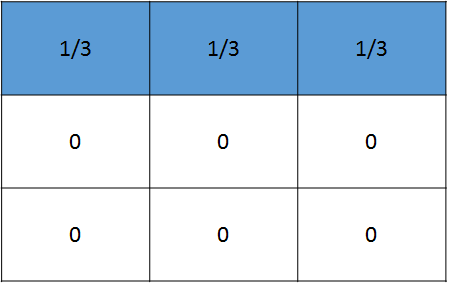
\includegraphics[width=0.4\textwidth]{Z_stab_dps.png}}
		\subfloat[An eigenstate of $\omega^{-2^{-1}}ZX$]{\label{fig:stabps_b}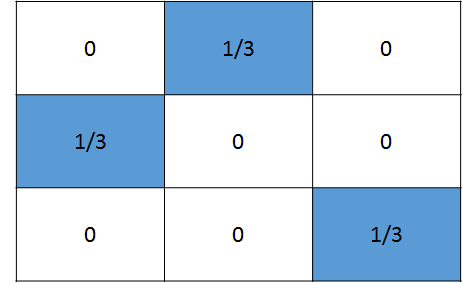
\includegraphics[width=0.4\textwidth]{XZ_stab_dps.png}}\\
		\subfloat[A typical non-stabilizer state]{\label{fig:stabps_c}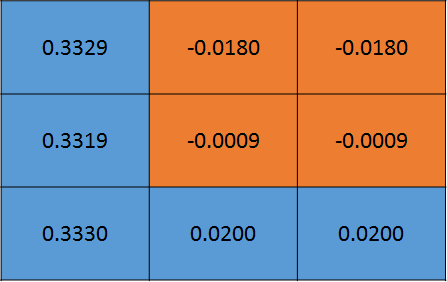
\includegraphics[width=0.4\textwidth]{rand_dps.png}}
		\caption[Discrete phase space and stabilizer states]{The stabilizer states form a line in the discrete phase space ($d = 3$ shown), while non-stabilizer states do not.}
	\end{center}
\end{figure}

Alice can specify what state $x$ is by sending Bob four integers (indicating two coordinates in the discrete phase space that have non-zero values) since they uniquely determine a line. Bob then knows exactly what state Alice has. Using \Cref{fig:stabps_a} for example, Alice could send (0,0) and (0,1) to Bob (the northwest and north points in the grid), and he would know for certain which eigenstate of the $Z$ matrix $x$ was. In Problem 2 specifically, since Clifford matrices map stabilizer states to stabilizer states, $Ux$ will form a line in the phase space, and Bob can send four integers back to Alice that specify two non-zero elements. Having $U$ and $x$ in the stabilizer sub-theory ensures a simple and effective way of solving both Problem 1 and Problem 2.

\subsection{Communication Complexity of the Protocols}
\label{subsec:complexity}
Without considering the precision on the mana values, \Cref{tab:step_complex} shows the maximum communication complexity of each step in Protocols 1 and 2. The communication complexity behaves like $O(T_1$ log $d)$ for Protocol 1 and $O(T_2$ log $d)$ for Protocol 2. Given the analysis of repetitions required for each protocol in \Cref{subsec:convergence_repetitions}, the complexities for each problem can be stated concisely. This is done in \Cref{tab:protocol_complex1,tab:protocol_complex2}.\\

\begin{table}[h]
\begin{center}
\begin{tabular}{r | c | c}
	\textbf{Step No.} & \textbf{Protocol 1} & \textbf{Protocol 2}\\\hline
	Step 1 & 0 bits & 0 bits \\\hline
	Step 2 & 2 log$d$ bits & 2 log$d$ bits \\\hline
	Step 3 & 0 bits& 2 log$d$ bits \\\hline
	Step 4 & 0 bits & 0 bits\\\hline
	Step 5 & $T_1$ times & 0 bits \\\hline
	Step 6 & 0 bits & $T_2$ times\\\hline
	Step 7 & N/A & 0 bits \\\hline
\end{tabular}
\end{center}
	\caption{Communication complexity of each step in the two protocols.}
	\label{tab:step_complex}
\end{table}

\begin{table}[h]
\begin{center}
\begin{tabular}{l | p{0.2\textwidth} | p{0.2\textwidth}}
	& {\bfseries Stabilizer $x$} & \textbf{General $x$}\\\hline
	\textbf{Protocol 1}
		& $\bullet$ $O($log $d)$\newline $\bullet$ 1 round
		& $\bullet$ $O(d$ log $d)$\newline $\bullet$ $d$ rounds \\\hline
	\textbf{Quantum Solution 1}
		& $\bullet$ $O($log $d)$\newline $\bullet$ 1 round
		& $\bullet$ $O($log $d)$\newline $\bullet$ 1 round \\\hline
	\textbf{Raz's Solution}
		& $\bullet$ $O(\sqrt{d})$
		& $\bullet$ $O(\sqrt{d})$ \\\hline
\end{tabular}
\end{center}
	\caption[Communication complexity of protocols for Problem 1.]{Communication complexity and number of rounds for each protocol that solves Problem 1 in specified input cases.}
	\label{tab:protocol_complex1}
\end{table}

\begin{table}[h]
\begin{center}
\begin{tabular}{p{0.18\textwidth} | p{0.15\textwidth} | p{0.13\textwidth} | p{0.15\textwidth} | p{0.14\textwidth}}
	& {\bfseries Stabilizer $x$, Clifford $U$}
		& \textbf{General $x$, Clifford $U$}
		& \textbf{Stabilizer $x$, General $U$}
		& \textbf{General $x$, General $U$}\\\hline
	\textbf{Protocol 2}
		& $\bullet$ $O($log $d)$\newline $\bullet$ 1 round
		& $\bullet$ $O(d$ log $d)$\newline $\bullet$ $d$ rounds
		& $\bullet$ $O(d^2$ log $d)$\newline $\bullet$ $d^2$ rounds
		& $\bullet$ $O(d^3$ log $d)$\newline $\bullet$ $d^3$ rounds \\\hline
	\textbf{Quantum\,\,\,\, Solution 2}
		& $\bullet$ $O($log $d)$\newline $\bullet$ 2 rounds
		& $\bullet$ $O($log $d)$\newline $\bullet$ 2 rounds
		& $\bullet$ $O($log $d)$\newline $\bullet$ 2 rounds
		& $\bullet$ $O($log $d)$\newline $\bullet$ 2 rounds \\\hline
	\textbf{Raz's Solution}
		& $\bullet$ $O(d^{3/4})$
		& $\bullet$ $O(d^{3/4})$
		& $\bullet$ $O(d^{3/4})$
		& $\bullet$ $O(d^{3/4})$ \\\hline
\end{tabular}
\end{center}
	\caption[Communication complexity of protocols for Problem 2.]{Communication complexity and number of rounds for each protocol that solves Problem 2 in specified input cases.}
	\label{tab:protocol_complex2}
\end{table}

In order to keep the complexities listed, $\hat{\mathcal{M}}_U(\alpha)$ and $\hat{\mathcal{M}}_\rho$ must be transmitted in $O($log $d)$ bits, or less, for each case. For unsigned real numbers (which can be used as the mana is always positive), this can be done using the Institute of Electrical and Electronics Engineers (IEEE) convention, since the mana is always bounded above by $d$. For example, if a number $a$ can be expressed as $a = c2^q, c,q \in \mathbb{Z}$, by restricting $c$ to be an integer 3 log $d$ digits long and $q \in [0, 2$ log $d]$, $a$ can be any real value between 1 and $d$ (to some finite precision), which is all that is required for specifying the mana. These two integers, $c$ and $q$, can be expressed in $O($log $d)$ bits. Thus, Alice and Bob can communicate these mana values while achieving high precision and without altering the overall communication complexity of the protocols.

\end{document}